\documentclass[oneside,openany,headings=optiontotoc,11pt,numbers=noenddot]{scrreprt}

\usepackage[a4paper]{geometry}
\usepackage[utf8]{inputenc}
\usepackage[T1]{fontenc}
\usepackage{lmodern}
\usepackage[ngerman]{babel}
\usepackage{ngerman}

\usepackage[onehalfspacing]{setspace}

\usepackage{fancyhdr}
\usepackage{fancybox}

\usepackage{rotating}
\usepackage{varwidth}

%Struktogramme
\usepackage[german,curves]{struktex}

\usepackage{pdflscape}
\usepackage{changepage}
\usepackage{graphicx}
\usepackage[bottom]{footmisc}
\usepackage{transparent}
\usepackage{graphbox}
\graphicspath{
	{Pics/PDFs/}
	{Pics/JPGs/}
	{Pics/PNGs/}
}
\usepackage{caption}
\usepackage{wrapfig}
\usepackage{marginnote}
\usepackage{tabularx}
\usepackage{dashrule}
\usepackage{soulutf8}
\usepackage{hhline}
%arydshln suppresses vertical lines in table
%\usepackage{arydshln}
\usepackage{multirow}
\usepackage{enumerate}
\usepackage[hidelinks]{hyperref}
\usepackage{listings}

\usepackage[table]{xcolor}
\usepackage{array}
\usepackage{enumitem,amssymb,amsmath}
\usepackage{interval}
\usepackage{cancel}
\usepackage{stmaryrd}
\usepackage{wasysym}
\usepackage{polynom}
\usepackage{diagbox}
\usepackage{dashrule}
\usepackage{framed}
\usepackage{mdframed}
\usepackage{karnaugh-map}
\usepackage{pdfpages}

\usepackage{blindtext}

\usepackage{eso-pic}

\usepackage{amssymb}
\usepackage{eurosym}

\usepackage[pages=some]{background}
\pagestyle{headings}
\renewcommand{\headrulewidth}{0.2pt}
\renewcommand{\footrulewidth}{0.2pt}
\newcommand*{\underdownarrow}[2]{\ensuremath{\underset{\overset{\Big\downarrow}{#2}}{#1}}}
\setlength{\fboxsep}{5pt}
\newcommand{\explainBelow}[3]{\underbrace{#1}_{\parbox{\widthof{#3}}{\footnotesize\raggedright #2}}}
\newcommand{\explainAbove}[3]{\overbrace{#1}^{\parbox{\widthof{#3}}{\footnotesize\raggedright #2}}}
\newcommand\footnoteref[1]{\protected@xdef\@thefnmark{\ref{#1}}\@footnotemark}


% Codestyle defined
\definecolor{codegreen}{rgb}{0,0.6,0}
\definecolor{codegray}{rgb}{0.5,0.5,0.5}
\definecolor{codepurple}{rgb}{0.58,0,0.82}
\definecolor{backcolour}{rgb}{0.95,0.95,0.92}
\definecolor{deepgreen}{rgb}{0,0.5,0}
\definecolor{darkblue}{rgb}{0,0,0.65}
\definecolor{mauve}{rgb}{0.40, 0.19,0.28}
\colorlet{exceptioncolour}{yellow!50!red}
\colorlet{commandcolour}{blue!60!black}
\colorlet{numpycolour}{blue!60!green}
\colorlet{specmethodcolour}{violet}

%Neue Spaltendefinition
\newcolumntype{L}[1]{>{\raggedright\let\newline\\\arraybackslash\hspace{0pt}}m{#1}}
\newcolumntype{M}{>{\centering\arraybackslash}X}
\newcommand{\cmnt}[1]{\ignorespaces}
%Textausrichtung ändern
\newcommand\tabrotate[1]{\rotatebox{90}{\raggedright#1\hspace{\tabcolsep}}}

%Intervall-Konfig
\intervalconfig {
	soft open fences
}

%Bash
\lstdefinestyle{BashInputStyle}{
	language=bash,
	basicstyle=\small\sffamily,
	backgroundcolor=\color{backcolour},
	columns=fullflexible,
	backgroundcolor=\color{backcolour},
	breaklines=true,
}
%Java
\lstdefinestyle{JavaInputStyle}{
	language=Java,
	backgroundcolor=\color{backcolour},
	aboveskip=1mm,
	belowskip=1mm,
	showstringspaces=false,
	columns=flexible,
	basicstyle={\footnotesize\ttfamily},
	numberstyle={\tiny},
	numbers=none,
	keywordstyle=\color{purple},,
	commentstyle=\color{deepgreen},
	stringstyle=\color{blue},
	emph={out},
	emphstyle=\color{darkblue},
	emph={[2]rand},
	emphstyle=[2]\color{specmethodcolour},
	breaklines=true,
	breakatwhitespace=true,
	tabsize=2,
}
%Python
\lstdefinestyle{PythonInputStyle}{
	language=Python,
	alsoletter={1234567890},
	aboveskip=1ex,
	basicstyle=\footnotesize,
	breaklines=true,
	breakatwhitespace= true,
	backgroundcolor=\color{backcolour},
	commentstyle=\color{red},
	otherkeywords={\ , \}, \{, \&,\|},
	emph={and,break,class,continue,def,yield,del,elif,else,%
		except,exec,finally,for,from,global,if,import,in,%
		lambda,not,or,pass,print,raise,return,try,while,assert},
	emphstyle=\color{exceptioncolour},
	emph={[2]True,False,None,min},
	emphstyle=[2]\color{specmethodcolour},
	emph={[3]object,type,isinstance,copy,deepcopy,zip,enumerate,reversed,list,len,dict,tuple,xrange,append,execfile,real,imag,reduce,str,repr},
	emphstyle=[3]\color{commandcolour},
	emph={[4]ode, fsolve, sqrt, exp, sin, cos, arccos, pi,  array, norm, solve, dot, arange, , isscalar, max, sum, flatten, shape, reshape, find, any, all, abs, plot, linspace, legend, quad, polyval,polyfit, hstack, concatenate,vstack,column_stack,empty,zeros,ones,rand,vander,grid,pcolor,eig,eigs,eigvals,svd,qr,tan,det,logspace,roll,mean,cumsum,cumprod,diff,vectorize,lstsq,cla,eye,xlabel,ylabel,squeeze},
	emphstyle=[4]\color{numpycolour},
	emph={[5]__init__,__add__,__mul__,__div__,__sub__,__call__,__getitem__,__setitem__,__eq__,__ne__,__nonzero__,__rmul__,__radd__,__repr__,__str__,__get__,__truediv__,__pow__,__name__,__future__,__all__},
	emphstyle=[5]\color{specmethodcolour},
	emph={[6]assert,range,yield},
	emphstyle=[6]\color{specmethodcolour}\bfseries,
	emph={[7]Exception,NameError,IndexError,SyntaxError,TypeError,ValueError,OverflowError,ZeroDivisionError,KeyboardInterrupt},
	emphstyle=[7]\color{specmethodcolour}\bfseries,
	emph={[8]taster,send,sendMail,capture,check,noMsg,go,move,switch,humTem,ventilate,buzz},
	emphstyle=[8]\color{blue},
	keywordstyle=\color{blue}\bfseries,
	rulecolor=\color{black!40},
	showstringspaces=false,
	stringstyle=\color{deepgreen}
}

\lstset{literate=%
	{Ö}{{\"O}}1
	{Ä}{{\"A}}1
	{Ü}{{\"U}}1
	{ß}{{\ss}}1
	{ü}{{\"u}}1
	{ä}{{\"a}}1
	{ö}{{\"o}}1
}

% Neue Klassenarbeits-Umgebung
\newenvironment{worksheet}[3]
% Begin-Bereich
{
	\newpage
	\sffamily
	\setcounter{page}{1}
	\ClearShipoutPicture
	\AddToShipoutPicture{
		\put(55,761){{
				\mbox{\parbox{385\unitlength}{\tiny \color{codegray}BBS I Mainz, #1 \newline #2
						\newline #3
					}
				}
			}
		}
		\put(455,761){{
				\mbox{\hspace{0.3cm}
\includegraphics[width=0.2\textwidth]{../../logo.pdf}}
			}
		}
	}
}
% End-Bereich
{
	\clearpage
	\ClearShipoutPicture
}

\geometry{left=2.50cm,right=2.50cm,top=3.00cm,bottom=1.00cm,includeheadfoot}

\begin{document}
	\begin{worksheet}{BGY 16}{Mathematik - Lernbereich 3, Algebraisierung}{Übungsaufgabe zu Länge eines Vektors und Winkel zwischen Vektoren}
		
		\begin{framed}
			\noindent
			\tiny{\color{codegray}S. 102 Aufgabe 11}\\
			\normalsize
			\noindent
			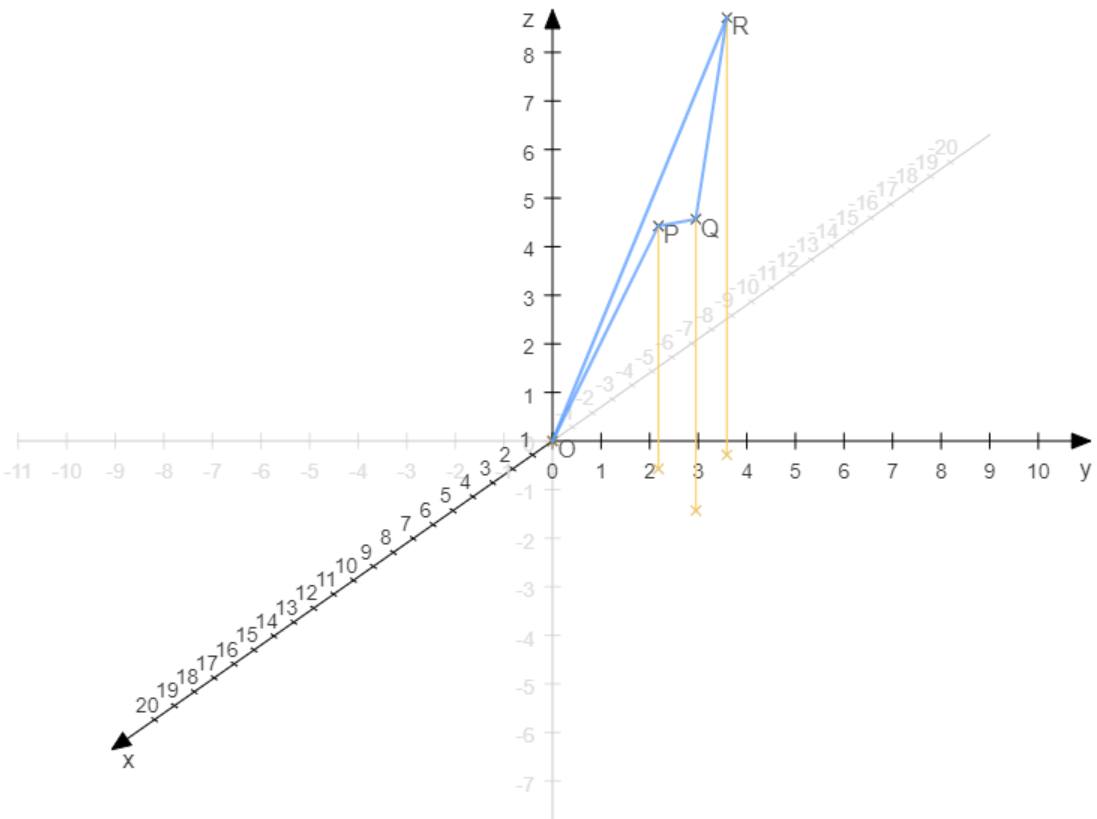
\includegraphics[scale=0.7]{Bilder/S102N11.png}\\
			Gegeben war das Viereck mit den Eckpunkten O (0 | 0 | 0), P (2 | 3 | 5), Q (5 | 5 | 6) und R (1 | 4 | 9).\\
			\par\noindent
			Zur Berechnung der Länge der Seiten benötigen wir die Verbindungsvektoren.\\
			Da die Formel \(cos{(\alpha)} = \frac{\vec{a}*\vec{b}}{|\vec{a}|*|\vec{b}|}\) sich auf den eingeschlossenen Winkel bezieht, benötigen wir jeweils die einschließenden Verbindungsvektoren.\(^{1}\)\\
			\tiny{\color{codegray}Es gilt: \(\vec{OP} = \vec{P}-\vec{O}\).}\\
			\normalsize
			\par\noindent
			\begin{tabularx}{\textwidth}{XXXX}
				%OP
				\(\vec{OP} = \left(\begin{array}{c}2 \\ 3 \\5\end{array}\right)\) &
				%PQ
				\(\vec{PQ} =\left(\begin{array}{c}3\\2\\1\end{array}\right)\) &
				%QR
				\(\vec{QR}=\left(\begin{array}{c}-4\\-1\\3\end{array}\right)\) &
				%RO
				\(\vec{RO}=\left(\begin{array}{c}-1\\-4\\-9\end{array}\right)\)\\
				%PO
				\(\vec{PO}= \left(\begin{array}{c}-2\\-3 \\-5\end{array}\right)\) &
				%QP
				\(\vec{QP}=\left(\begin{array}{c}-3\\-2\\-1\end{array}\right)\) &
				%RQ
				\(\vec{RQ}=\left(\begin{array}{c}4\\1\\-3\end{array}\right)\)&
				%OR
				\(\vec{OR}=\left(\begin{array}{c}1\\4\\9\end{array}\right)\)
			\end{tabularx}
			\\
			\par\noindent
			\tiny{\color{codegray}Da innerhalb der Längenberechnung die Koordinatenwerte quadriert werden gilt \(|\vec{OP}| = |\vec{PO}|\). Es genügt also jeweils einmal die Länge zu berechnen.}\\\noindent
			\normalsize
			Wir berechnen also zunächst die Längen der einzelnen Seiten.\\
			\par\noindent
			\begin{tabularx}{\textwidth}{XX}
				\(|\vec{OP}| = \sqrt{4+9+25} \approx 6,16\) & \(|\vec{PQ}| = \sqrt{9 + 4 + 1} \approx 3,74\)\\
				\(|\vec{QR}| = \sqrt{16 + 1 + 9} \approx 5,1\) & \(|\vec{RO}| = \sqrt{1 + 16 + 81} \approx 9,9 \)
			\end{tabularx}
		\par\bigskip\noindent
		\small{\color{codegray}[1] Siehe hierzu (*) auf der Rückseite.}
		\newpage
		\noindent
		Um nun den Winkel zu berechnen, benötigen wir zum einen die oben erwähnte Formel bzw. deren Umkehrfunktion.\\
		Diese geht wie folgt: \(\alpha = \arccos{\frac{\vec{a}*\vec{b}}{|\vec{a}|*|\vec{b}|}}\)\\
		\par
		\(\angle{ROP} = \arccos{\frac{\vec{OP}*\vec{OR}}{|\vec{OP}|*|\vec{OR}|}} =\arccos{\frac{2*1 + 3*4 + 5*9}{6,16*9,9}} \approx 14,65^{\circ}\)\\
		\par\noindent
		Bei der Berechnung des Winkels \(\angle{OPQ}\) ist zu beachten, dass wir den Außenwinkel benötigen. Die uns bekannte Formel aber immer den eingeschlossenen Winkel berechnet. Wir rechnen also \(360^{\circ}-\angle{OPQ}\). (*)\\
		\par
		\(360^{\circ} - \angle{OPQ} = 360^{\circ} -  \arccos{\frac{\vec{PO}*\vec{PQ}}{|\vec{PO}|*|\vec{PQ}|}} =360^{\circ} - \arccos{\frac{3*(-2)+2*(-3)+1*(-5)}{6,16*3,74}} \approx 222,45^{\circ}\)\\
		\par
		\(\angle{PQR} = \arccos{\frac{\vec{QP}*\vec{QR}}{|\vec{QP}|*|\vec{QR}|}} =\arccos{\frac{(-3)*(-4)+(-2)*(-1)+(-1)*3}{3,74*5,1}} \approx 54,80^{\circ}\)\\
		\par
		\(\angle{QRO} = \arccos{\frac{\vec{RQ}*\vec{RO}}{|\vec{RQ}|*|\vec{RO}|}} =\arccos{\frac{4*(-1)+1*(-4)+(-3)*(-9)}{5,1*9,9}} \approx 67,89^{\circ}\)\\
		\par\bigskip\noindent
		In den uns bekannten Vierecken beträgt die Winkelsumme \(360^{\circ}\text{.}^{2}\) Um also zu prüfen, ob wir uns auch nicht verrechnet haben, addieren wir einfach alle Winkel zusammen.\\
		\[14,65^{\circ} + 222,45^{\circ} + 54,80^{\circ} + 67,89^{\circ} = 359,79^{\circ}\]\\
		Da wir die Längen und auch die Winkel auf zwei Nachkommastellen gerundet haben erhalten wir hier nicht ganz \(360^{\circ}\). Dennoch sehen wir, dass wir ziemlich nah dran sind!\\
		\par\noindent
		\small{\color{codegray}[2] Dass es Vierecke gibt, bei denen die Aussage nicht stimmt, zeigt Aufgabe 12 auf Seite 102.\\Wann genau das der Fall ist und wie man das prüft lernen wir im Laufe des Halbjahres.}
		\end{framed}
		\begin{framed}
			\noindent
			(*) Wir erinnern uns an die Formel zur Berechnung des Winkel zwischen zwei Vektoren.\\
			\centering
			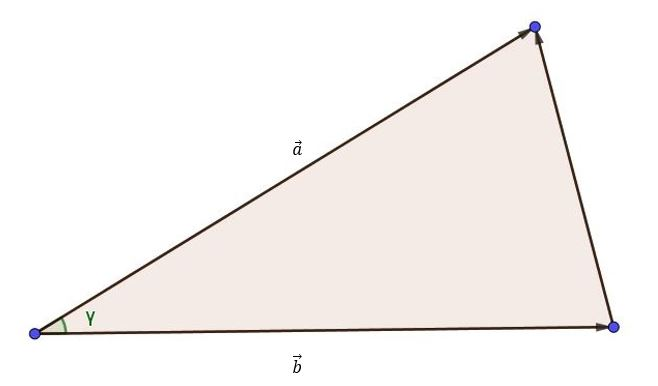
\includegraphics[scale=0.45]{Bilder/Dreieck.jpg}\\
			\raggedright
			Ist \(\gamma\) der von den Vektoren \(\vec{a}\) und \(\vec{b}\) eingeschlossene Winkel, so lässt sich der dazugehörige \(\cos\) wie folgt bestimmen
			\[\cos(\gamma) = \frac{\vec{a}*\vec{b}}{|\vec{a}|*|\vec{b}|} = \frac{a_1*b_1 + a_2*b_2 + a_3*b_3}{\sqrt{a_1^2 + a_2^2 + a_3^2}*\sqrt{b_1^2 + b_2^2 + b_3^2}}\]\\
			Um daraus den Winkel \(\gamma\) zu bestimmen, verwenden wir die Umkehrfunktion \(\arccos \widehat{=}cos^{-1}\).
			\[\gamma = \arccos{\frac{\vec{a}*\vec{b}}{|\vec{a}|*|\vec{b}|}} = \arccos{\frac{a_1*b_1 + a_2*b_2 + a_3*b_3}{\sqrt{a_1^2 + a_2^2 + a_3^2}*\sqrt{b_1^2 + b_2^2 + b_3^2}}}\]
		\end{framed}
	\end{worksheet}
\end{document}